% !TEX root = main.tex
\chapter{Thực nghiệm và đánh giá hệ thống}

\section{Thực nghiệm và đánh giá mô hình phân loại}
\subsection{Các tiêu chí đánh giá}
Để đánh giá mô hình dự đoán, hệ thống sẽ sử dụng tập dữ liệu test đã được tạo ra từ trước (766 mẫu). Các tiêu chí đánh giá bao gồm 4 thành phần sau:
\subsubsection{Độ chính xác (Precision)}
Precision là tỉ lệ số mẫu dương thực tế (Positive) so với tổng số mẫu mà mô hình dự đoán là dương, cho biết mô hình dự đoán một kết quả là "đúng" với độ tin cậy
là bao nhiêu.
\begin{equation}
	\mathrm{Precision} = \frac{TP}{TP + FP}
\end{equation}
Trong đó, $TP$ là số mẫu dương được dự đoán đúng và $FP$ là số mẫu âm bị dự đoán nhầm thành dương.

\subsubsection{Độ bao phủ (Recall)}
Độ bao phủ là tỉ lệ mà mô hình dự đoán là dương tính so với các mẫu vốn dĩ, chắc chắn là dương, cho biết mô hình bỏ sót bao nhiêu mẫu thực tế cần tìm
\begin{equation}
	\mathrm{Recall} = \frac{TP}{TP + FN}
\end{equation}
Trong đó, $FN$ là số mẫu dương bị dự đoán nhầm thành âm.

\subsubsection{Điểm F1 (F1-score)}
F1-score là trung bình điều hòa của Precision và Recall, giúp đánh giá cân bằng giữa độ chính xác và độ bao phủ khi dữ liệu bị mất cân bằng.
\begin{equation}
	\mathrm{F1\text{-}score} = 2 \times \frac{\mathrm{Precision} \times \mathrm{Recall}}{\mathrm{Precision} + \mathrm{Recall}}
\end{equation}

\subsubsection{Đường cong ROC (ROC Curve)}
ROC Curve là một đồ thị biểu diễn khả năng phân loại của mô hình tại các ngưỡng (threshold) khác nhau.

\subsection{Kết quả thực nghiệm}
\subsubsection{Bảng kết quả}
\begin{figure}[H]
    \centering
    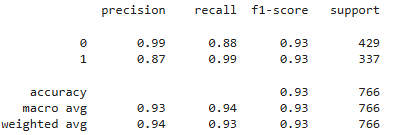
\includegraphics[width=0.6\textwidth]{images/chapter_04/img_33.png}
    \caption{Bảng kết quả thống kê}
    \label{fig:nlp}
\end{figure}

\noindent
Ta có thể thấy mô hình đạt độ chính xác lên tới 93\% và F1-score của hai lớp đều như nhau cũng với 93\%. Ngoài ra, precision rất cao đối với lớp Human và recall
cao đối với AI, cho thấy mô hình dự đoán các văn bản thuộc AI rất tốt nhưng recall của Human hơi thấp hơn (88\%), cho thấy các văn bản Human vẫn bị dự đoán nhầm thành AI.

\subsubsection{Ma trận sai lầm}
\begin{figure}[H]
    \centering
    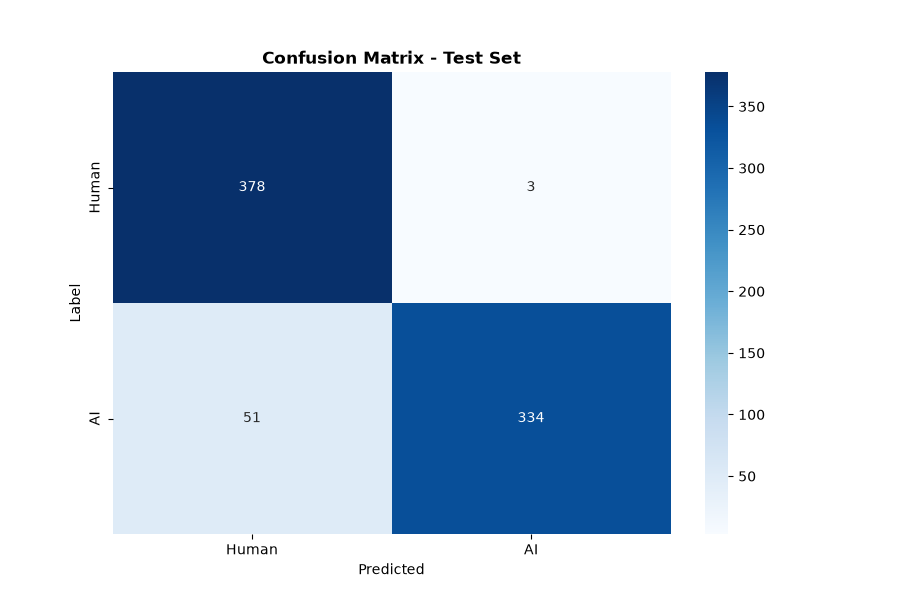
\includegraphics[width=0.8\textwidth]{images/chapter_04/img_34.png}
    \caption{Ma trận sai lầm}
    \label{fig:nlp}
\end{figure}

\noindent
Cụ thể số liệu như sau, qua ma trận nhầm lẫn trên. Ta có thể thấy trong 429 bài báo thì có 378 là dự đoán đúng là Human và 3 bài còn lại dự đoán nhầm là AI. Bên cạnh đó, trong
337 bài thì có 51 bài là AI mà dự đoán nhầm là Human và chỉ dự đoán đúng 334 bài AI còn lại.

\subsubsection{Độ chính xác của ba phương pháp sinh dữ liệu}
\begin{figure}[H]
    \centering
    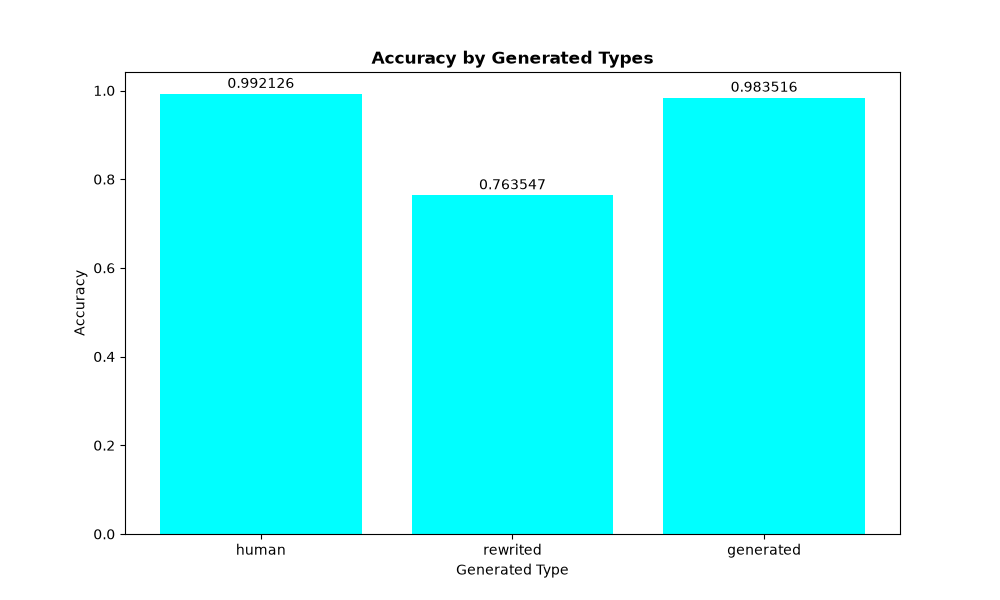
\includegraphics[width=0.9\textwidth]{images/chapter_04/img_35.png}
    \caption{Độ chính xác của ba phương pháp sinh dữ liệu}
    \label{fig:nlp}
\end{figure}

\noindent
Độ chính xác của ba phương pháp tạo dữ liệu như sau: Human: 99\%, AI-Generated: 98\% và AI-Rewrited: 76\%. Điều này cho thấy độ chính xác của mô hình trên tập test tốt nhưng vẫn dự 
đoán sai các văn bản được AI viết lại, độ chính xác thấp hơn hẳn so với hai nhóm còn lại.

\subsubsection{Đường cong ROC}
\begin{figure}[H]
    \centering
    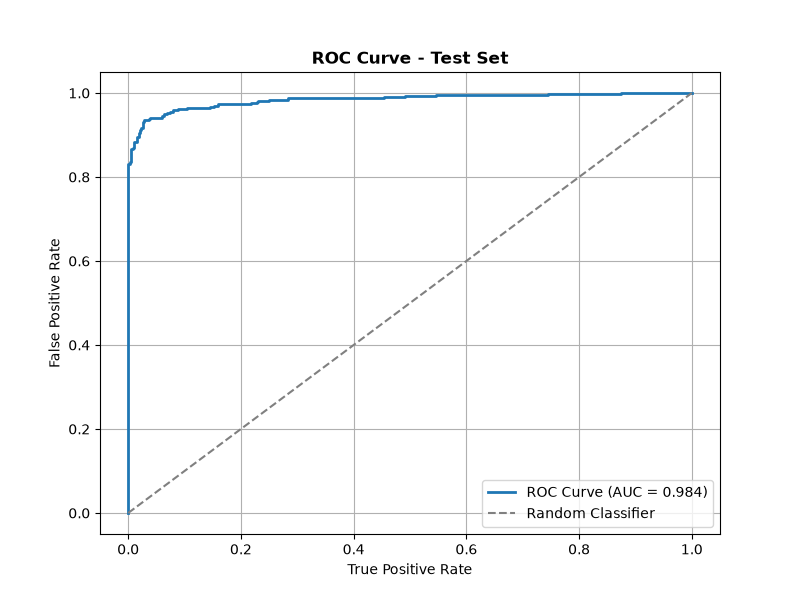
\includegraphics[width=0.8\textwidth]{images/chapter_04/img_36.png}
    \caption{Đường cong ROC}
    \label{fig:nlp}
\end{figure}

\noindent
Đường cong ROC cũng cho thấy mô hình phân biệt tốt hai lớp với độ chính xác rất cao, giá trị AUC lên tới 98\%, là đường cong nằm gần góc trái, mô hình càng dự đoán chính xác thì đường cong càng
gần góc trái hơn, tức là độ bao phủ trên tập dữ liệu lớn hơn.

\section{Đánh giá thuật toán giải thích Integrated Gradients}
\subsection{Đánh giá hội tụ và độ trung thực của giải thích}
\begin{figure}[H]
    \centering
    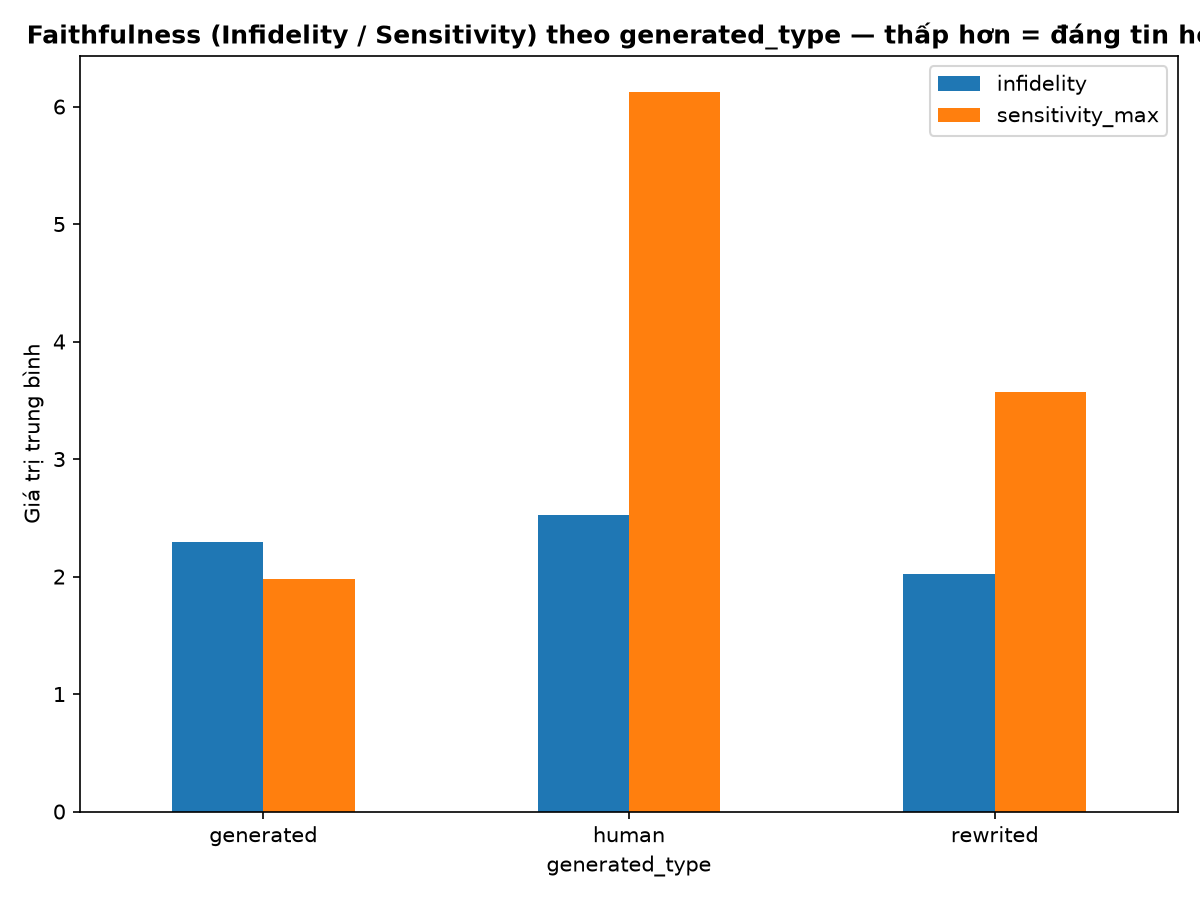
\includegraphics[width=0.8\textwidth]{images/chapter_04/img_37.png}
    \caption{Độ bất trung thực và Độ ổn định}
    \label{fig:nlp}
\end{figure}

\noindent
Độ bất trung thực (Infidelity) sẽ cho biết các điểm attribution có phản ánh đúng mức độ đầu ra của token hay từ đến đầu ra của mô hình hay không, tức là khi ta thay đổi hay bỏ một từ mà điểm attribution cao (từ đó
có mức độ ảnh hưởng lớn đến kết quả) thì đầu ra của mô hình cũng phải thay đổi đáng kể. Infidelity thấp là tốt, vì điều đó cho thấy attribution dự đoán đúng mức độ thay đổi của mô hình khi đầu vào bị thay đổi. Ví dụ, ta xét một chuỗi câu sau: ``I love AI'' và giả sử mô hình trả về xác suất văn bản do AI tạo ra là $0.90$.

\begin{itemize}
    \item \textbf{Trường hợp giải thích tốt:} attribution của token ``AI'' là $+0.70$. Khi thay token này bằng một token trung tính hoặc loại bỏ token, xác suất dự đoán giảm từ $0.90$ xuống $0.35$, tức là thay đổi $0.55$. Mức attribution cao đã phản ánh đúng ảnh hưởng lớn của token ``AI'', nên sai lệch giữa attribution và thay đổi thực tế nhỏ; do đó Infidelity thấp.
    \item \textbf{Trường hợp giải thích kém:} attribution của token ``love'' là $+0.35$. Tuy nhiên, khi thay hoặc loại bỏ token này, xác suất dự đoán chỉ giảm từ $0.90$ xuống $0.89$, tức là thay đổi $0.01$. Mặc dù attribution cho rằng token ``love'' có ảnh hưởng đáng kể, đầu ra của mô hình gần như không thay đổi. Vì vậy, sai lệch lớn và Infidelity cao, cho thấy giải thích không trung thực.
\end{itemize}

Độ nhạy (Sensitivity) cho biết mức độ ổn định của attribution khi đầu vào có sự thay đổi nhẹ, tức là nếu đầu vào có thay đổi một chút thì liệu các attribution score có thay đổi đáng kể hay không. Ví dụ, ta xét một chuỗi sau: "AI đang phát triển mạnh trong lĩnh vực công nghệ."

\begin{itemize}
    \item \textbf{Trường hợp giải thích ổn định:} với câu gốc, attribution của các token ``AI'', ``phát triển'' và ``công nghệ'' lần lượt là $+0.40$, $+0.25$ và $+0.15$. Khi thay token ``mạnh'' bằng ``rất mạnh'', các attribution tương ứng chỉ thay đổi nhẹ, chẳng hạn thành $+0.39$, $+0.26$ và $+0.14$. Vì đầu vào chỉ thay đổi một token nhưng cách mô hình giải thích gần như được giữ nguyên, Sensitivity thấp và đây là kết quả tốt.
    \item \textbf{Trường hợp giải thích không ổn định:} với cùng thay đổi nhỏ ``mạnh'' thành ``rất mạnh'', attribution của các token trên lại thay đổi mạnh, chẳng hạn từ $+0.40$, $+0.25$, $+0.15$ thành $-0.10$, $+0.65$, $+0.02$. Khi đó, một thay đổi nhỏ trong câu đã làm mô hình phân bổ mức độ ảnh hưởng sang các token khác một cách đáng kể. Sensitivity cao, cho thấy attribution thiếu ổn định và giải thích không đáng tin cậy.
\end{itemize}

Qua hình 38, ta có thể thấy giá trị infidelity trung bình của ba nhóm tương đối gần nhau và thấp, dao động từ 2 - 2.5, trong đó nhóm \texttt{rewrited} đạt giá trị thấp nhất. Điều này cho thấy mức độ trung thực của nhóm \texttt{rewrited} tốt hơn so với hai nhóm còn lại. Ngoài ra, đối với sensitivity thì nhóm \texttt{generated} đạt giá trị thấp nhất (xấp xỉ 2.0), cho thấy tính ổn định của nhóm \texttt{generated} tốt hơn so với hai nhóm còn lại nhưng
nhóm Human thì cao nhất (6.0), cho thấy attribution của nhóm này thay đổi đáng kể khi thay đổi nhỏ đầu vào.

\subsection{Phân tích kết quả attribution}
Sau đây là kết quả attribution score của các token tương ứng với bài báo của ba phương pháp tạo dữ liệu:

\begin{figure}[H]
    \centering
    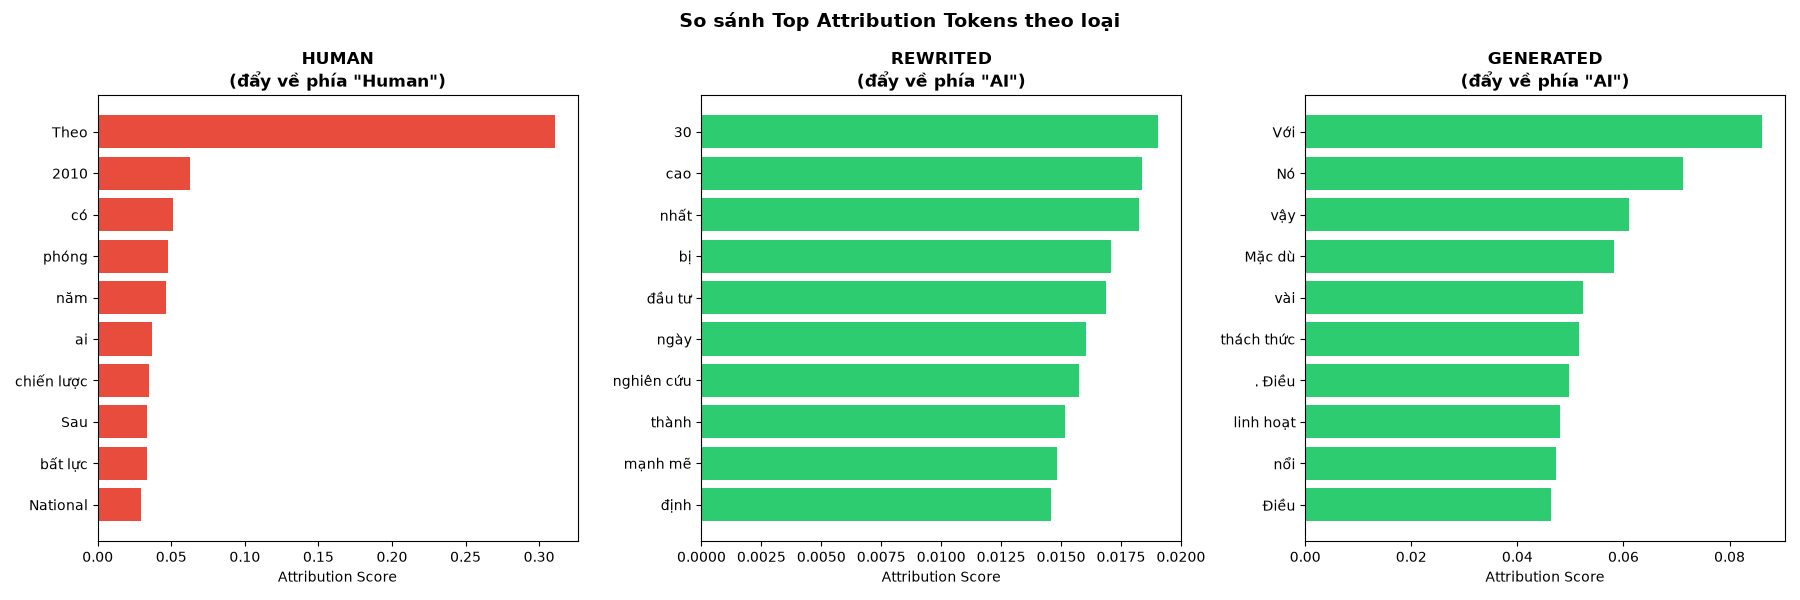
\includegraphics[width=1.0\textwidth]{images/chapter_04/img_38.png}
    \caption{Attribution score của các token tương ứng với ba phương pháp tạo dữ liệu}
    \label{fig:nlp}
\end{figure}

\section{Đánh giá kết quả giải thích bằng LLM}
\subsection{Thiết lập sinh giải thích}
\begin{Verbatim}[fontsize=\small, frame=single, rulecolor=\color{gray!20}, formatcom=\color{black}]
PROMPT_TEMPLATE = """
Bạn là trợ lý giải thích kết quả của một mô hình phát hiện văn bản AI tiếng Việt.
Model đã dự đoán: {predicted_class} (xác suất {pred_prob:.1%}).

Bằng chứng đã tính được (KHÔNG được suy đoán thêm ngoài các số liệu này):
- Từ ảnh hưởng mạnh nhất ủng hộ AI: {top_ai_words}
- Từ ảnh hưởng mạnh nhất ủng hộ Human: {top_human_words}
- Số câu: {sentence_count}, độ dài câu trung bình: {avg_sentence_length:.1f} từ, độ lệch chuẩn: {sentence_length_std:.1f}
- Mật độ dấu câu: {punctuation_density:.3f}

Trả lời CHÍNH XÁC theo định dạng dưới đây, MỖI BULLET TRÊN MỘT DÒNG MỚI:
- Giải thích đầu tiên
- Giải thích thứ hai
- Giải thích thứ ba
(và cứ như vậy, tối đa 5 bullet)

Giải thích vì sao văn bản có đặc điểm trên, CHỈ dựa trên các số liệu đã cho, không thêm thông tin ngoài dữ liệu này.
"""
\end{Verbatim}
\captionof{listing}{Prompt để sinh giải thích bằng LLM}
Ta có thể thấy, để ép LLM dựa trên số liệu tính được của thuật toán, mô hình thì yêu cầu (prompt) phải ràng buộc các đơn vị đo lường như: độ dài câu, độ lệch chuẩn của câu,
mật độ dấu câu, độ dài trung bình câu kết hợp với các top từ được mô hình dự đoán trên mỗi loại nhãn (AI/Human).

\begin{table}[H]
    \centering
    \caption{Thống kê kiểm tra mức độ bám sát số liệu của LLM}
    \label{tab:llm-groundedness}
    \small
    \renewcommand{\arraystretch}{1.2}
    \setlength{\tabcolsep}{5pt}
    \begin{tabular}{c c c c c}
        \toprule
        \begin{tabular}[c]{@{}c@{}}\texttt{known\_words}\\\texttt{referenced}\end{tabular} &
        \begin{tabular}[c]{@{}c@{}}\texttt{known\_words}\\\texttt{total}\end{tabular} &
        \begin{tabular}[c]{@{}c@{}}\texttt{words}\\\texttt{ratio}\end{tabular} &
        \begin{tabular}[c]{@{}c@{}}\texttt{numeric\_claims}\\\texttt{matched}\end{tabular} &
        \begin{tabular}[c]{@{}c@{}}\texttt{numeric}\\\texttt{ratio}\end{tabular}
        \\
        \midrule
        6 & 8 & 0.75 & 2 & 0.67 \\
        5 & 6 & 0.83 & 2 & 0.67 \\
        8 & 10 & 0.80 & 1 & 0.33 \\
        10 & 12 & 0.83 & 2 & 0.67 \\
        8 & 9 & 0.89 & 3 & 1.00 \\
        8 & 8 & 1.00 & 2 & 0.67 \\
        10 & 10 & 1.00 & 3 & 1.00 \\
        10 & 14 & 0.71 & 3 & 1.00 \\
        10 & 12 & 0.83 & 2 & 0.67 \\
        10 & 10 & 1.00 & 3 & 1.00 \\
        \bottomrule
    \end{tabular}
\end{table}

\clearpage

\begin{table}[H]
    \centering
    \caption{Các chỉ số dấu câu và trạng thái kiểm tra của LLM}
    \label{tab:llm-punctuation-check}
    \small
    \renewcommand{\arraystretch}{1.2}
    \setlength{\tabcolsep}{5pt}

    \begin{tabular}{c c c c}
        \toprule
        \begin{tabular}[c]{@{}c@{}}\texttt{bullets\_punctuation}\\\texttt{density}\end{tabular} &
        \begin{tabular}[c]{@{}c@{}}\texttt{signals\_punctuation}\\\texttt{density}\end{tabular} &
        \begin{tabular}[c]{@{}c@{}}\texttt{punctuation}\\\texttt{match}\end{tabular} &
        \texttt{status} \\
        \midrule
        0.048 & 0.021 & 1.0 & \texttt{ok} \\
        0.042 & 0.019 & 1.0 & \texttt{ok} \\
        0.054 & 0.023 & 1.0 & \texttt{ok} \\
        0.053 & 0.016 & 1.0 & \texttt{ok} \\
        0.053 & 0.032 & 1.0 & \texttt{ok} \\
        0.054 & 0.029 & 1.0 & \texttt{ok} \\
        0.046 & 0.022 & 1.0 & \texttt{ok} \\
        0.046 & 0.026 & 1.0 & \texttt{ok} \\
        0.057 & 0.030 & 1.0 & \texttt{ok} \\
        0.060 & 0.021 & 1.0 & \texttt{ok} \\
        \bottomrule
    \end{tabular}
\end{table}

Trong đó, \texttt{known\_words\_referenced} là số từ hoặc đặc trưng đã được cung cấp mà LLM thực sự đề cập, còn \texttt{known\_words\_total} là tổng số từ hoặc đặc trưng được cung cấp trong prompt. Tương tự, \texttt{numeric\_claims\_matched} là số nhận định số học được LLM trích dẫn đúng và \texttt{numeric\_ratio} là tỉ lệ nhận định số học đúng trên tổng số nhận định cần kiểm tra. Hai cột \texttt{bullets\_punctuation\_density} và \texttt{signals\_punctuation\_density} lần lượt biểu thị mật độ dấu câu trong phần bullet do LLM sinh ra và trong số liệu đầu vào. \texttt{punctuation\_match} cho biết mức độ khớp giữa hai mật độ này. Giá trị \texttt{status = ok} cho biết mẫu vượt qua các điều kiện kiểm tra. Bảng cho thấy LLM nhìn chung sử dụng các từ khóa, số liệu và đặc trưng dấu câu được cung cấp, qua đó xác nhận prompt đã ràng buộc phần giải thích dựa trên bằng chứng thay vì cho phép mô hình tự suy đoán.
